% Created 2024-10-24 Thu 14:42
% Intended LaTeX compiler: xelatex

\documentclass[10pt]{beamer}

% fonts
\usepackage{ctex}
\usepackage{fontspec}
\setmainfont{Times New Roman}
\setmonofont{Inconsolata}
\setsansfont{Times New Roman}
\setCJKmainfont{SimSong}
\setCJKsansfont{SimSong}

\usepackage{amsfonts}
\usepackage{amsthm}
\usepackage{bm}
\usepackage{siunitx}
\usepackage{xcolor}

\usepackage{mathrsfs}
% commands
\newcommand{\mr}[1]{\mathrm{#1}}
\newcommand{\mb}[1]{\mathbf{#1}}
\newcommand{\mc}[1]{\mathcal{#1}}
\newcommand{\ms}[1]{\mathscr{#1}}

\usepackage{graphicx}
\usepackage{longtable}
\usepackage{wrapfig}
\usepackage{rotating}
\usepackage[normalem]{ulem}
\usepackage{amsmath}
\usepackage{amssymb}
\usepackage{capt-of}
\usepackage{hyperref}
\usepackage{etoolbox}
\usepackage{pgfopts}
\usepackage{booktabs}
\usepackage[scale=2]{ccicons}
\usetheme[block=fill, progressbar=frametitle]{metropolis}
\useoutertheme{infolines} % 采用 infoline
\useinnertheme{default}
\usecolortheme{custom} % 使用 custom 颜色主题
\setbeamertemplate{blocks}[rounded][shadow=false]
\setbeamertemplate{items}[circle] % circle item symbol
\setbeamertemplate{sections/subsections in toc}[ball] % ball section symbol
\setbeamertemplate{headline}[default] % 不使用 infoline 的 headline
%\setbeamertemplate{footline}[default] % 使用 infoline 的 footline
\setbeamertemplate{frame numbering}[none]
\setbeamertemplate{bibliography item}[text] % 使用 text 的 references 形式
%\setbeamerfont{footnote}{\tiny} % 可选择 tiny footnote
\usetheme{default}
\author{朱宇涛 \quad 报告人:王亚朋}
\date{2024年10月24日}
\title{余波, 能量刻度与 \(\mu\) 寿命测量}
\subtitle{宇宙线粒子探测与物理实验}

\hypersetup{
pdfauthor={朱宇涛 \quad 报告人:王亚朋},
pdftitle={余波, 能量刻度与 \(\mu\) 寿命测量},
pdfkeywords={},
pdfsubject={},
pdfcreator={Emacs 29.1 (Org mode 9.6.6)},
pdflang={Cn},
colorlinks=true,
linkcolor=black
}
\begin{document}

\maketitle
\begin{frame}[label={sec:org4131aa9}]{目录}
\tableofcontents
\end{frame}
\section{实验目标}
\label{sec:org2656d76}
\begin{frame}[label={sec:org6dd33f6}]{实验目标}
\begin{enumerate}
\item 重新测量暗噪声、电子学噪声、\(\mu\) 信号与余波的一些参数;
\item 测量单光子电荷;
\item 进行能量刻度;
\item 测量 \(\mu\) 寿命。
\end{enumerate}
\end{frame}
\section{实验结果}
\label{sec:orgc4cd6a9}
\begin{frame}[label={sec:org3d1d317}]{噪声}
在 1500V 电压下进行实验, 得到:
\begin{itemize}
\item 暗噪声频率 \(f_{d} \approx \qty{10.04}{Hz}\).
\item 电子学噪声振幅 \qty{0.5}{mV}.
\end{itemize}
\end{frame}

\begin{frame}[label={sec:orge0d7b3a}]{\(\mu\) 信号参数}
使用甄别器的 4、7 道(甄别电压 \qty{15}{mV}),测量符合信号。\footnote{后续实验条件不变.}

\begin{itemize}
\item 左:电压 1350V.

信号宽度:\(\Delta X(\mr{CH1}) = \qty{43.4}{ns}\).

计数率:\(n(\mr{CH1}) = \qty{2995}{min^{-1}}\).

\item 右:电压 1500V.

信号宽度:\(\Delta X(\mr{CH2}) = \qty{38.4}{ns}\).

计数率:\(n(\mr{CH2}) = \qty{2014}{min^{-1}}\).

\item 符合

计数率:\(n = \qty{859}{min^{-1}}\).
\end{itemize}

同时计算得到偶然符合计数率:
\begin{equation}
\label{eq:1}
n_a = \qty{0.176}{min^{-1}}.
\end{equation}
\end{frame}

\begin{frame}[label={sec:orge5b5599}]{余波时间分布}
\begin{columns}
\begin{column}{0.5\columnwidth}
\begin{figure}[htbp]
\centering
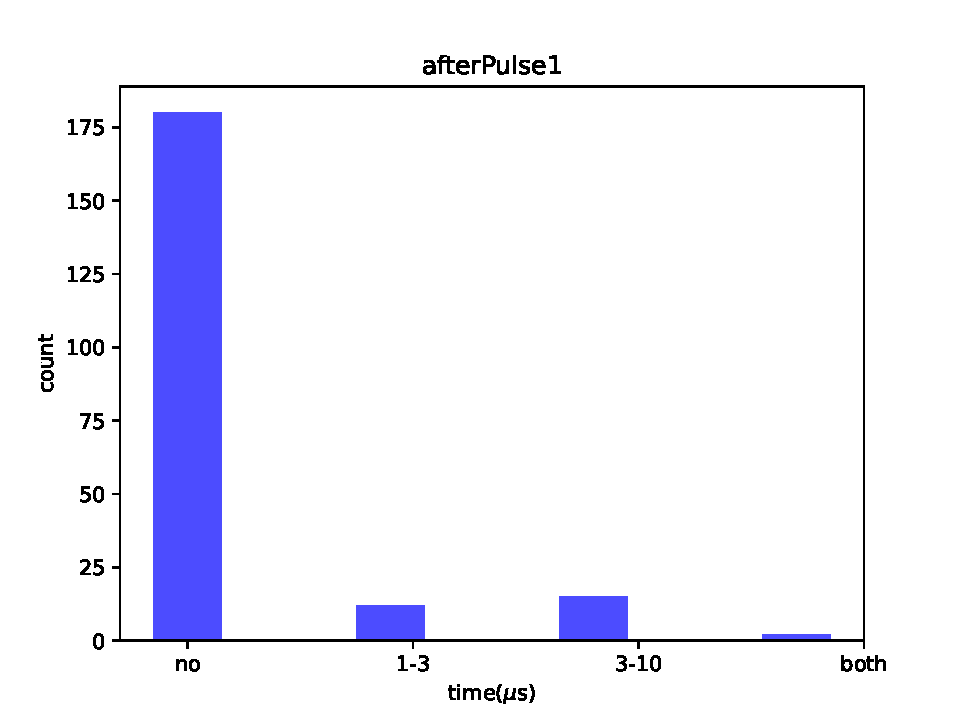
\includegraphics[width=1.0\textwidth]{../../img/afterPulse01.pdf}
\caption{所有信号的余波分布}
\end{figure}
\end{column}

\begin{column}{0.5\columnwidth}
\begin{figure}[htbp]
\centering
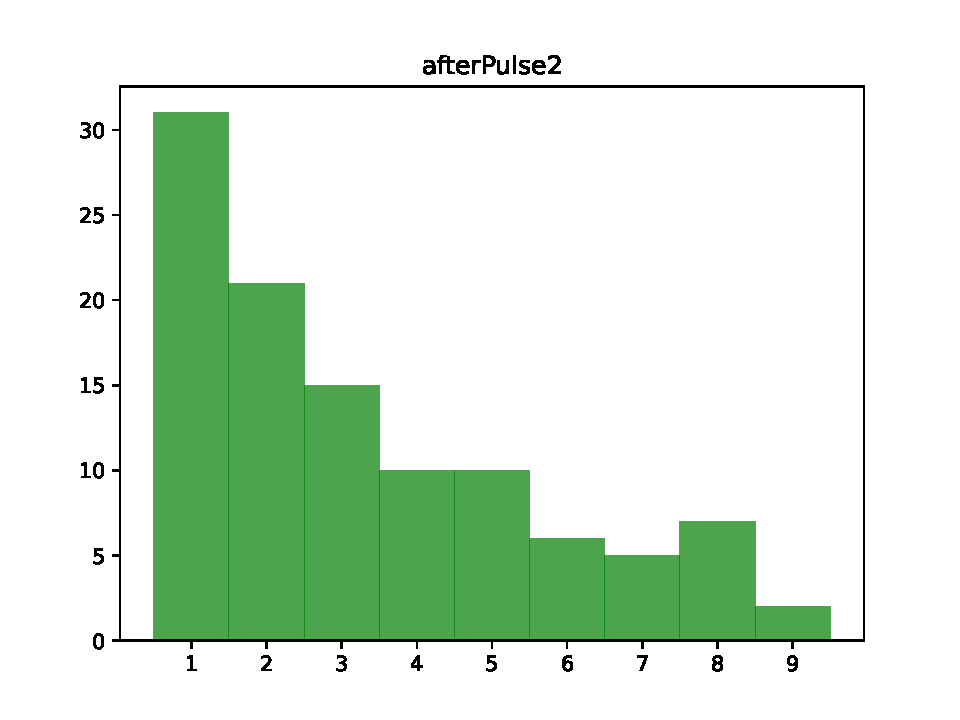
\includegraphics[width=1.0\textwidth]{../../img/afterPulse02.pdf}
\caption{存在余波信号的余波分布}
\end{figure}
\end{column}
\end{columns}
\end{frame}

\begin{frame}[label={sec:org407aa4f}]{余波时间分布}
对余波分布作指数拟合:

\begin{figure}[htbp]
\centering
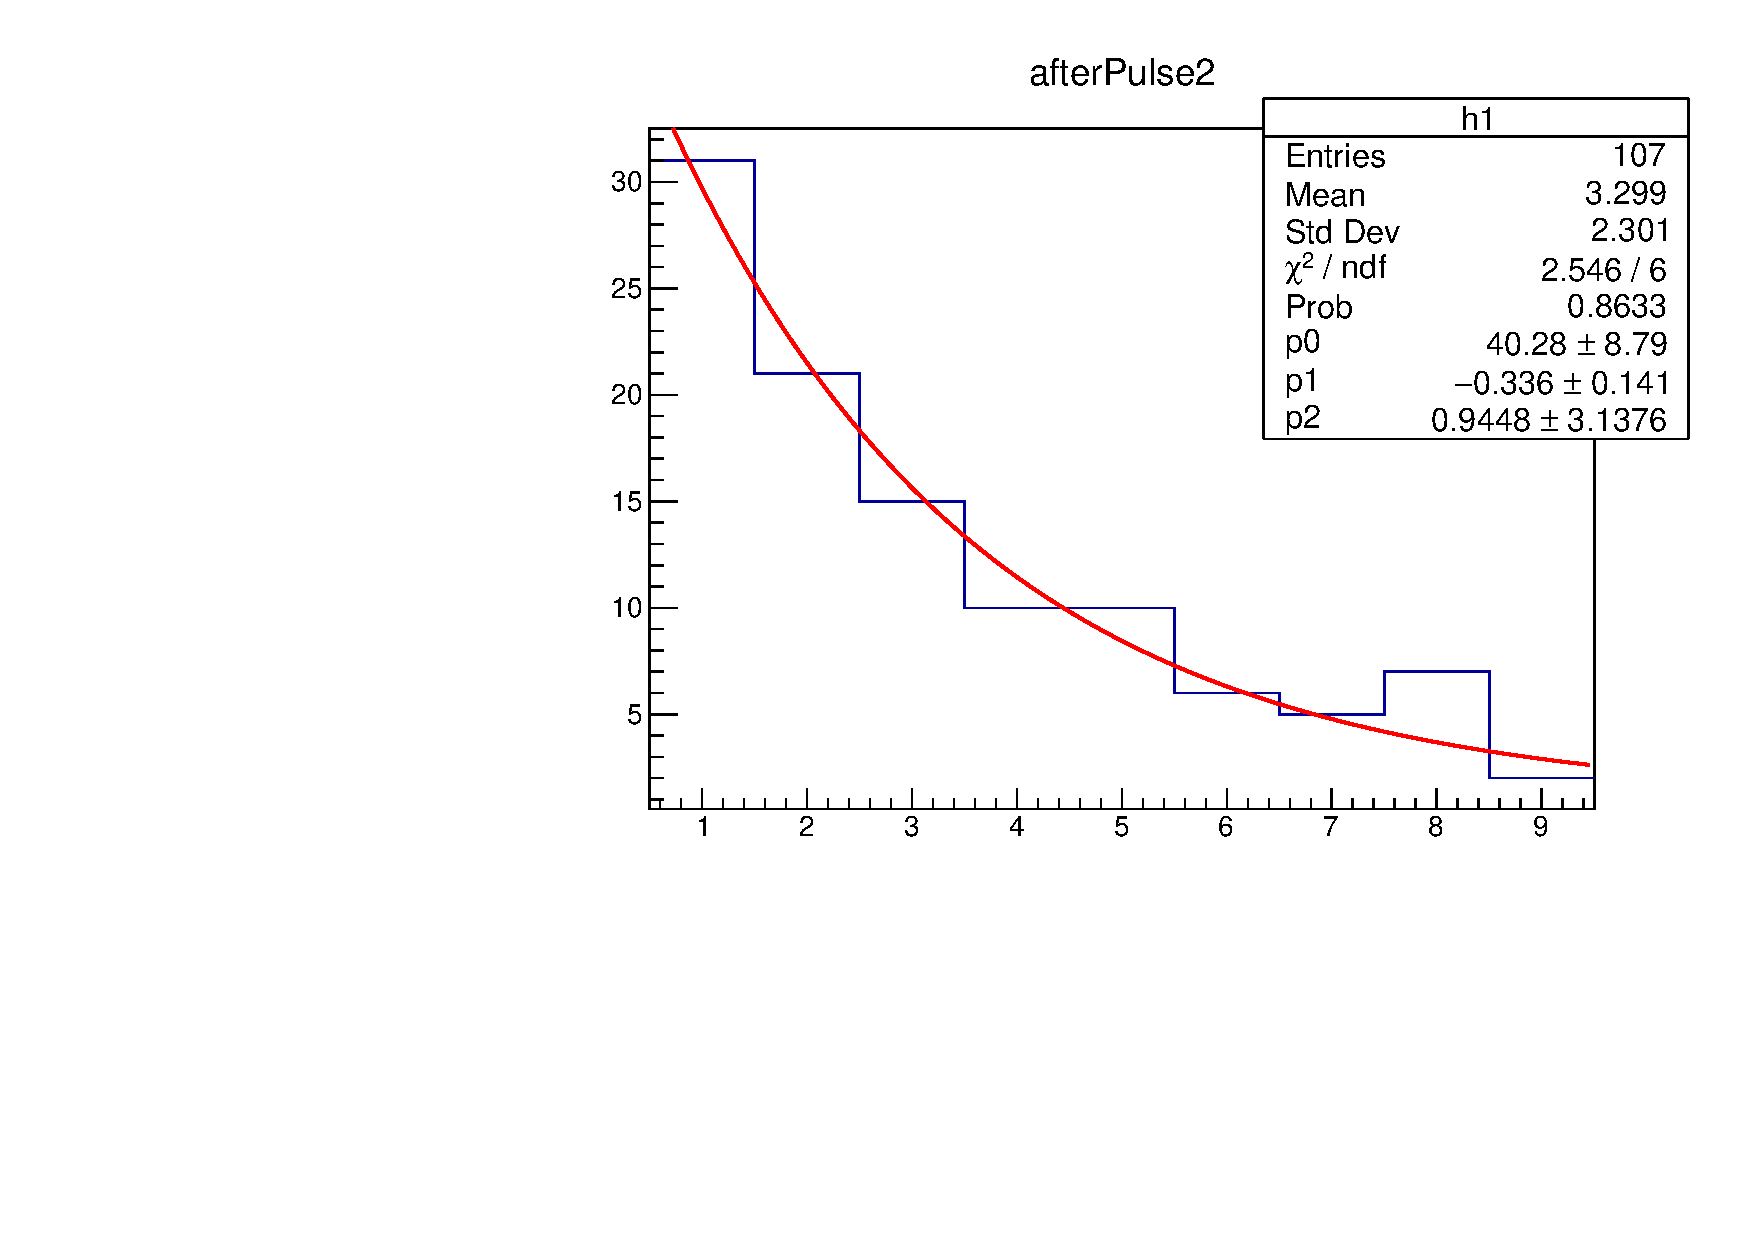
\includegraphics[width=0.7\textwidth]{../../img/afterPulse02r.pdf}
\caption{余波分布拟合}
\end{figure}
\end{frame}

\begin{frame}[label={sec:org84092e3}]{单光子电荷}
\begin{figure}[htbp]
\centering
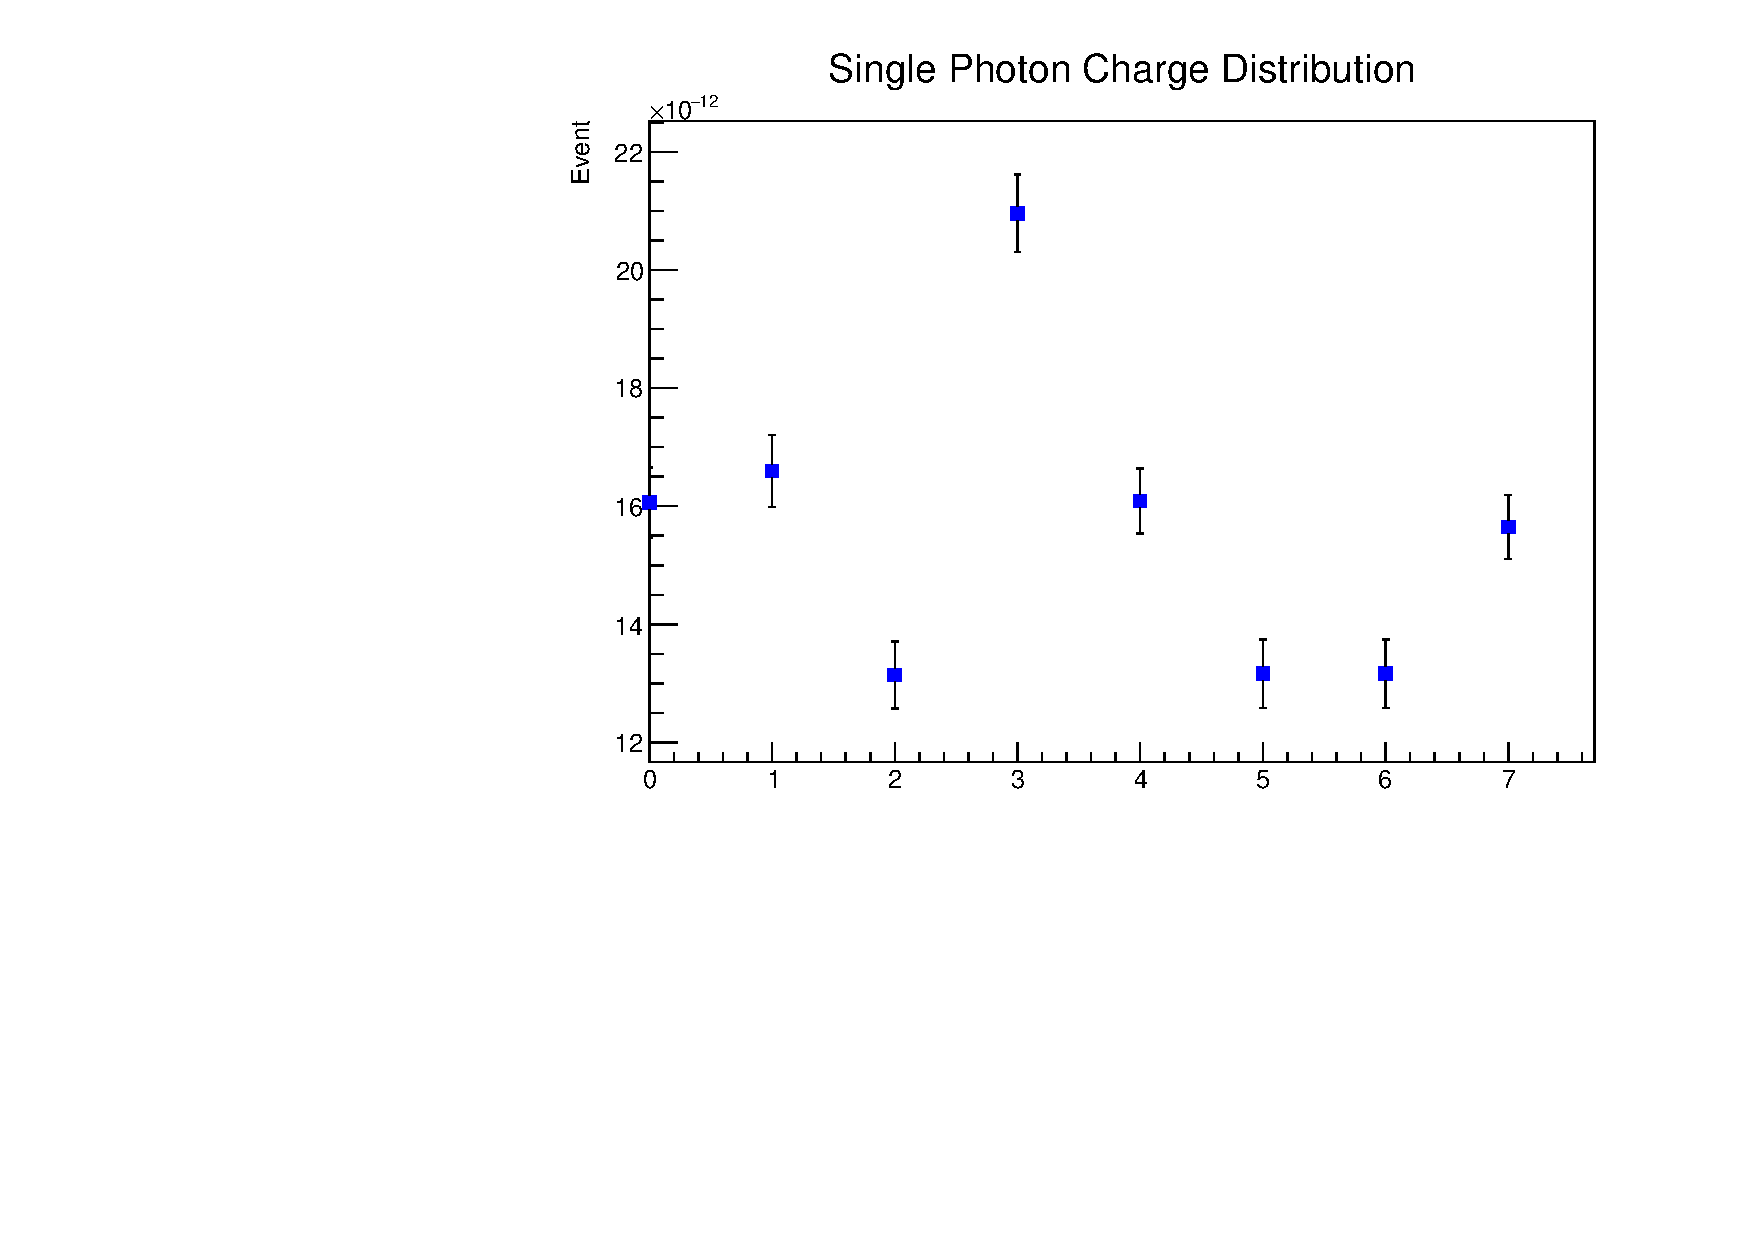
\includegraphics[width=0.6\textwidth]{../../DetectorPerform/SPhoton/SphotonCharge.pdf}
\caption{单光子电荷}
\end{figure}

单光子电荷量:
\begin{equation}
\label{eq:6}
q = (1.560 \pm 0.245)\times\qty{e-11}{V\cdot s}.
\end{equation}
\end{frame}

\begin{frame}[label={sec:org3adb80b}]{衰减长度}
考虑 Error Bar, 重新计算衰减长度\footnote{不确定度优于上次结果 (0.1494m).}与相关系数:
\begin{align}
\label{eq:3}
L &= 1.643 \pm \qty{0.131}{m} \\
\rho &= 0.442.
\end{align}

\begin{columns}
\begin{column}{0.5\columnwidth}
\begin{figure}[htbp]
\centering
\includegraphics[width=0.8\textwidth]{../../DetectorPerform/AttenuationLength/figs/Dist.png}
\caption{衰减长度}
\end{figure}
\end{column}

\begin{column}{0.5\columnwidth}
\begin{figure}[htbp]
\centering
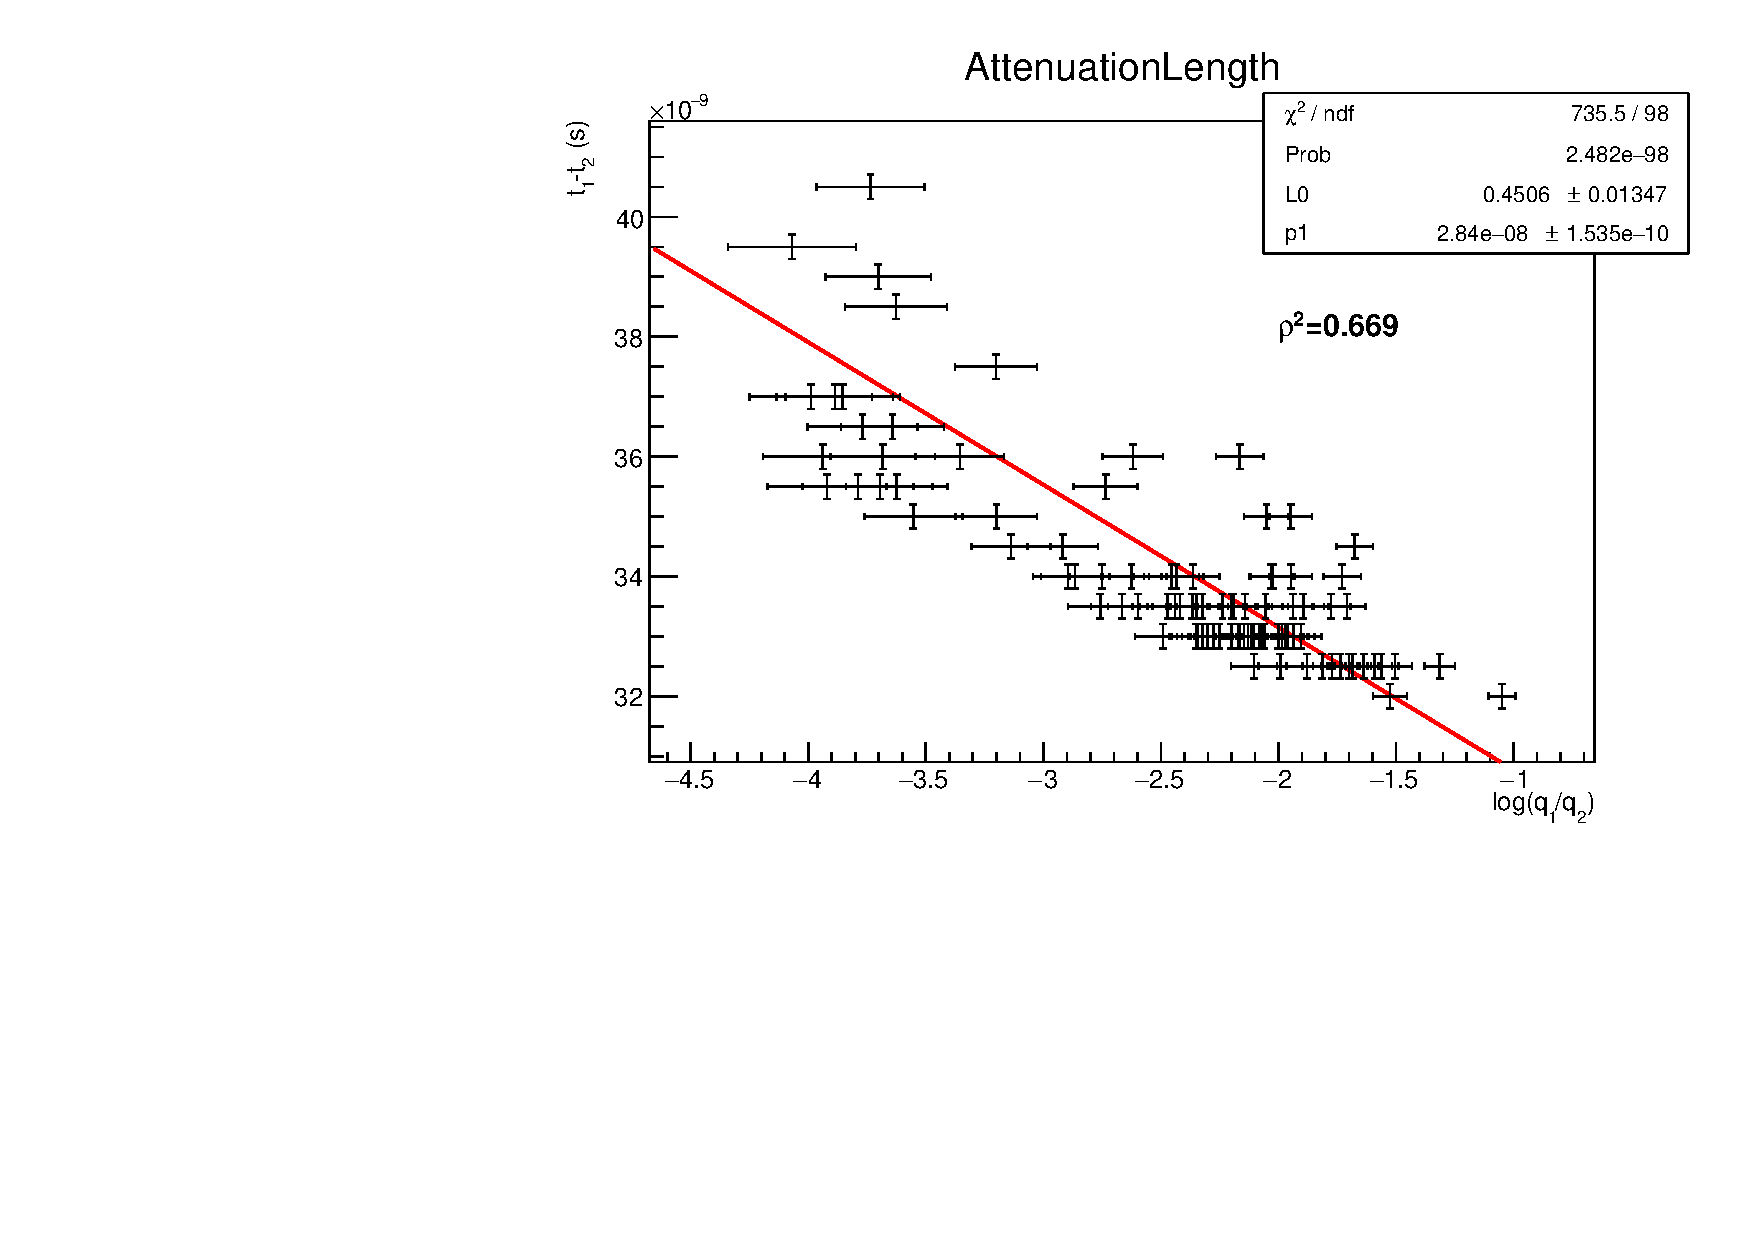
\includegraphics[width=0.8\textwidth]{../../DetectorPerform/AttenuationLength/figs/AttenuationLength.pdf}
\caption{衰减长度 (考虑 Error Bar)}
\end{figure}
\end{column}
\end{columns}
\end{frame}

\begin{frame}[label={sec:org2ad09ad}]{能量刻度}
\begin{figure}[htbp]
\centering
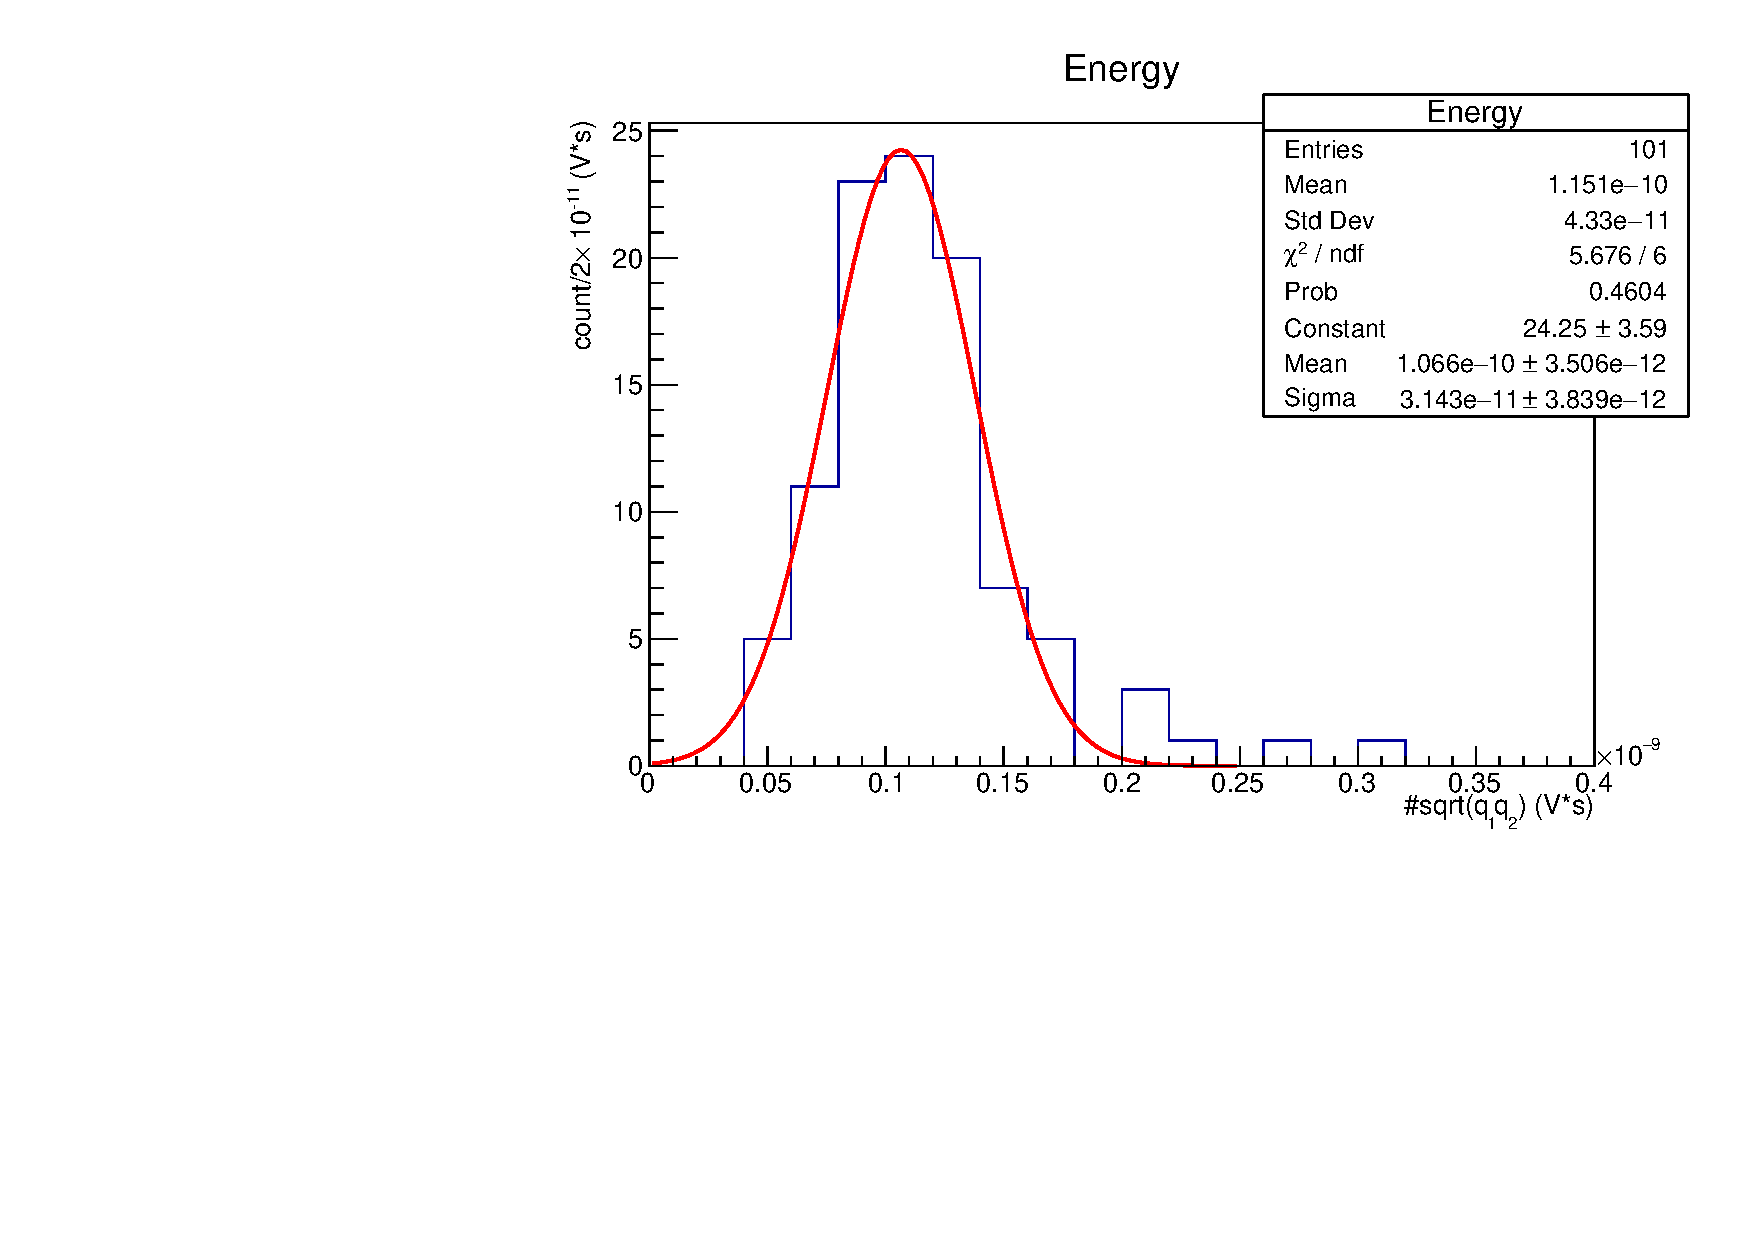
\includegraphics[width=0.5\textwidth]{../../DetectorPerform/ECali/qqdist.pdf}
\caption{能量刻度}
\end{figure}

能量分辨率为:
\begin{equation}
\label{eq:4}
\frac{2.35\sigma}{\mu} = \frac{\num{7.386e-11}}{\num{1.066e-10}} = 69.3\%.
\end{equation}
\end{frame}


\begin{frame}[label={sec:org07cdd48}]{\(\mu\) 寿命}
\begin{columns}
\begin{column}{0.5\columnwidth}
\begin{figure}[htbp]
\centering
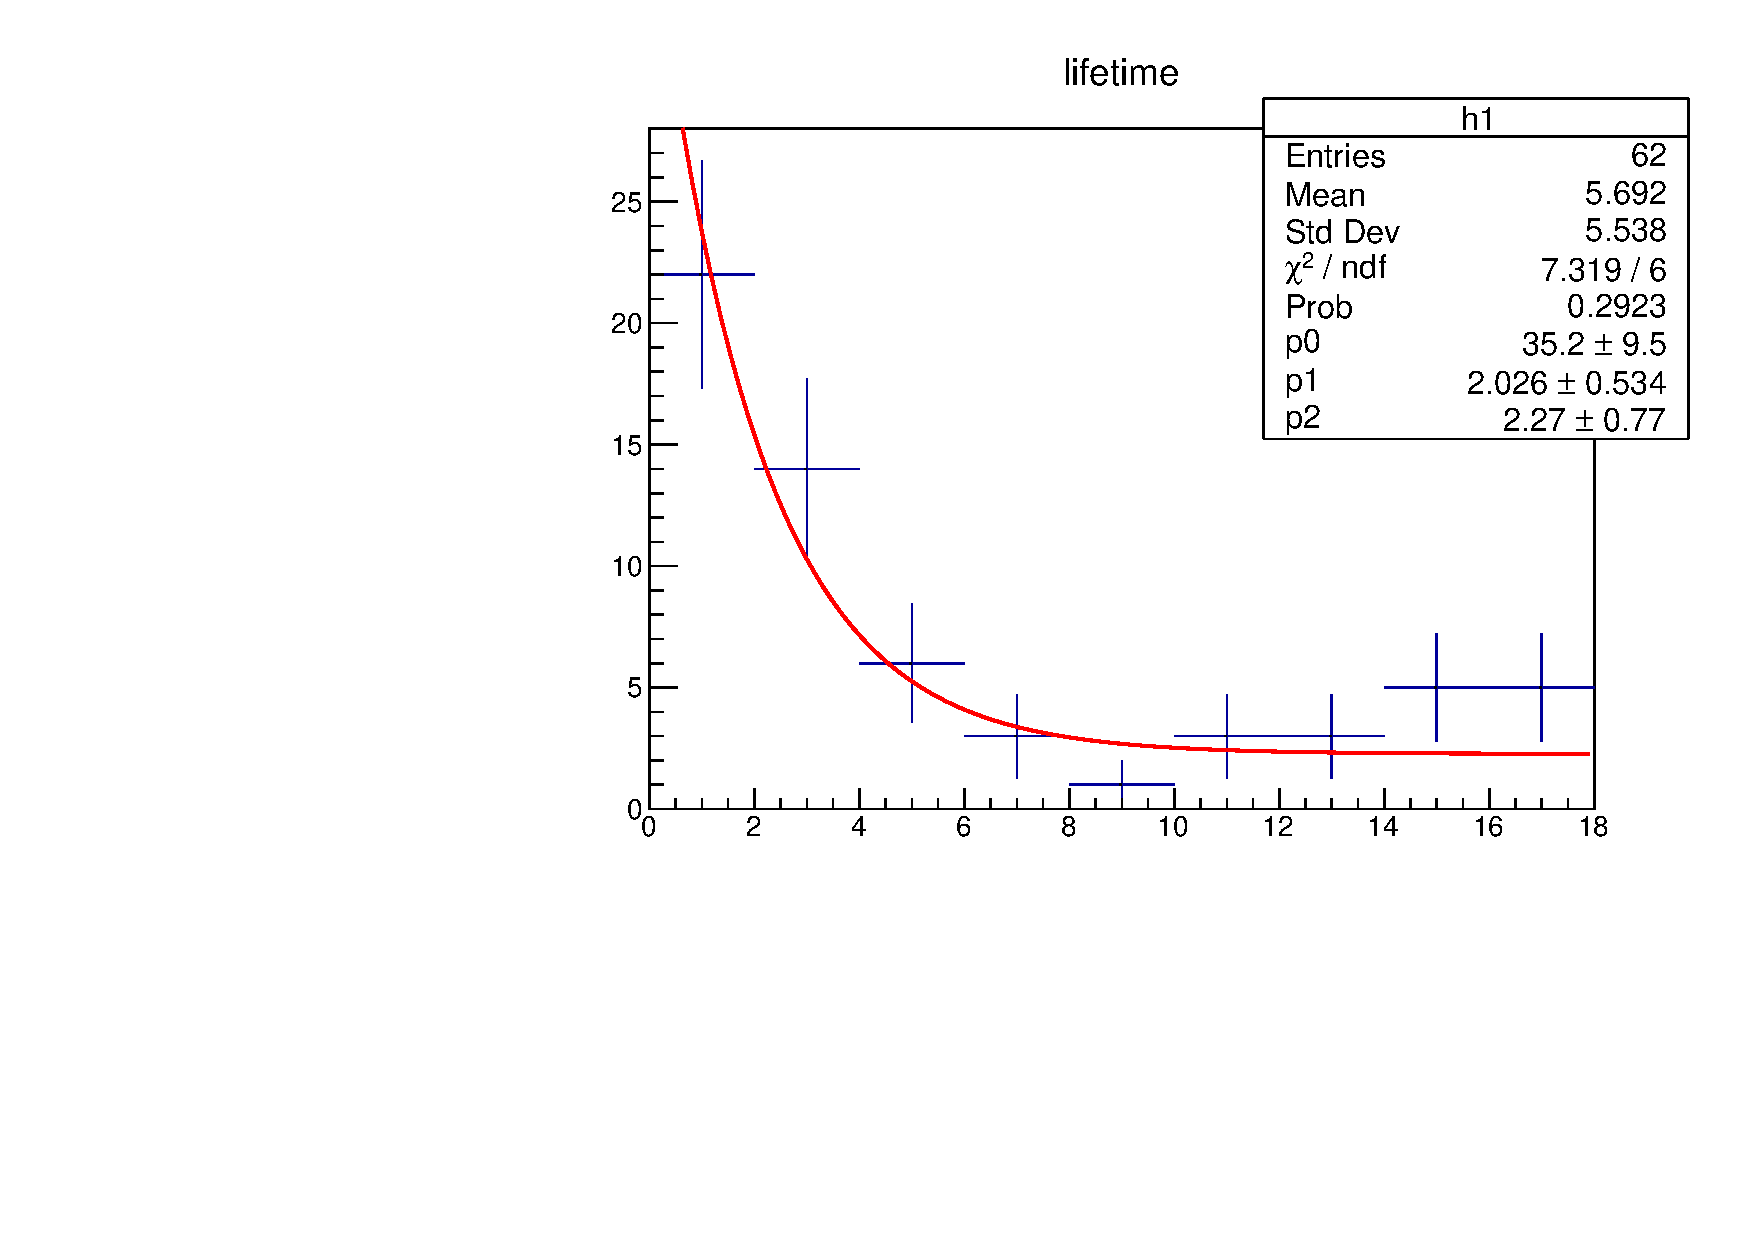
\includegraphics[width=1.0\textwidth]{../../img/lifeTimeHist.pdf}
\caption{\(\mu\) 寿命}
\end{figure}
\end{column}

\begin{column}{0.5\columnwidth}
测得 \(\mu\) 寿命:  
\begin{equation}
\label{eq:5}
\tau = 2.026 \pm \qty{0.534}{\mu s}.
\end{equation}
\end{column}
\end{columns}
\end{frame}
\end{document}